%************************************************
\chapter{Introduction}
\label{chp:Introduction}
%************************************************

%\section{Motion Vision}
%what is motion vision. what is the central question we want to answer ? Why do we try to answer above question using drosophila ?

\section{\protect\NoCaseChange{\textit{Drosophila}} as a model organism}
\textit{Drosophila melanogaster} is one of the most powerful model organisms available for functional dissection of neural circuits. It allows for most sophisticated in vivo neural manipulations - imaging, activation and suppression of neural activity. Over 100 years of research in \textit{Drosophila} has allowed generation of thousands of fly 'driver-lines' which can be used to express genes of interest in neuron-specific manner \parencite{Pfeiffer2008}. Along with this, \textit{Drosophila} allows several practical working advantages: They are small, has a short generation time of about 10 days and easy to grow in a lab. 

\textit{Drosophila} brain is estimated to contain about 100,000 neurons \parencite{Zheng2018}. \textit{Drosophila} brain involves computation of modest complexity. These computations are implemented in circuits that contain a limited number of neurons, and with \textit{Drosophila} genetic armoury almost each of these neuron can be precisely targeted. However even with comparatively less complexity, there are surprising parallels between how fly and mammalian brains process information \parencite{Borst2015}. Insights about the nervous system obtained in \textit{Drosophila} is thus often relevant for other species \parencite{Bellen2010, Venken2011}.

\section{Tools for functional dissection of \protect\NoCaseChange{\textit{Drosophila}} neural circuits}
To have a detailed understanding of how a neural circuit functions, we need to know role each individual neuron plays in that particular circuit. To achieve this, we would like to perform following three types of manipulations on the given neuron: (i) record neuronal activity from the neuron, (ii) activate the neuron and (iii) silence the neuron. Fortunately years of research in Drosophila has provided us with multiple tools in order to be able to perform these manipulations in the choice of neuron we want. The most important tool which enables us to do this in neuron-specific manner is the Gal4-UAS system (figure  \ref{fig:gal4uas}). 

\subsection{GAL4-UAS / LexA-lexAop}
Following the discovery of transposable DNA sequences (P-elements) in the \textit{Drosophila} genome \parencite{Rubin1982}, \cite{Brand1993} designed GAL4-UAS system. The GAL4-UAS system is the workhorse of \textit{Drosophila} genetics. The GAL4-UAS system is a binary expression system consisting of two main components: the yeast transcriptional factor GAL4 expressed in a specific pattern and a reporter gene under the control of UAS promoter that is silent in the absence of GAL4. Gal4-UAS system essentially involves crossing two fly lines: one called the 'driver-line', defines which neurons express required effector gene; the other called 'reporter-line', defines what gene is expressed in the neurons defined by driver line. 

Another independent binary transcriptional system which can be used is LexA-lexAop system. This method is based on the bacterial DNA-binding operator lexAop and controlled by the expression of LexA. LexA binds to and activates the lexA operator (lexAop). We can use LexA-lexAop system in combination with GAL4-UAS system to simultaneously express gene of interest in two different neuronal population. Using combination of GAL4-UAS and LexA-lexAop system, we can express following three types of reporter genes: Indicator, Suppressor \& Activator.
\begin{figure}
\centering
\hspace*{-1cm} 
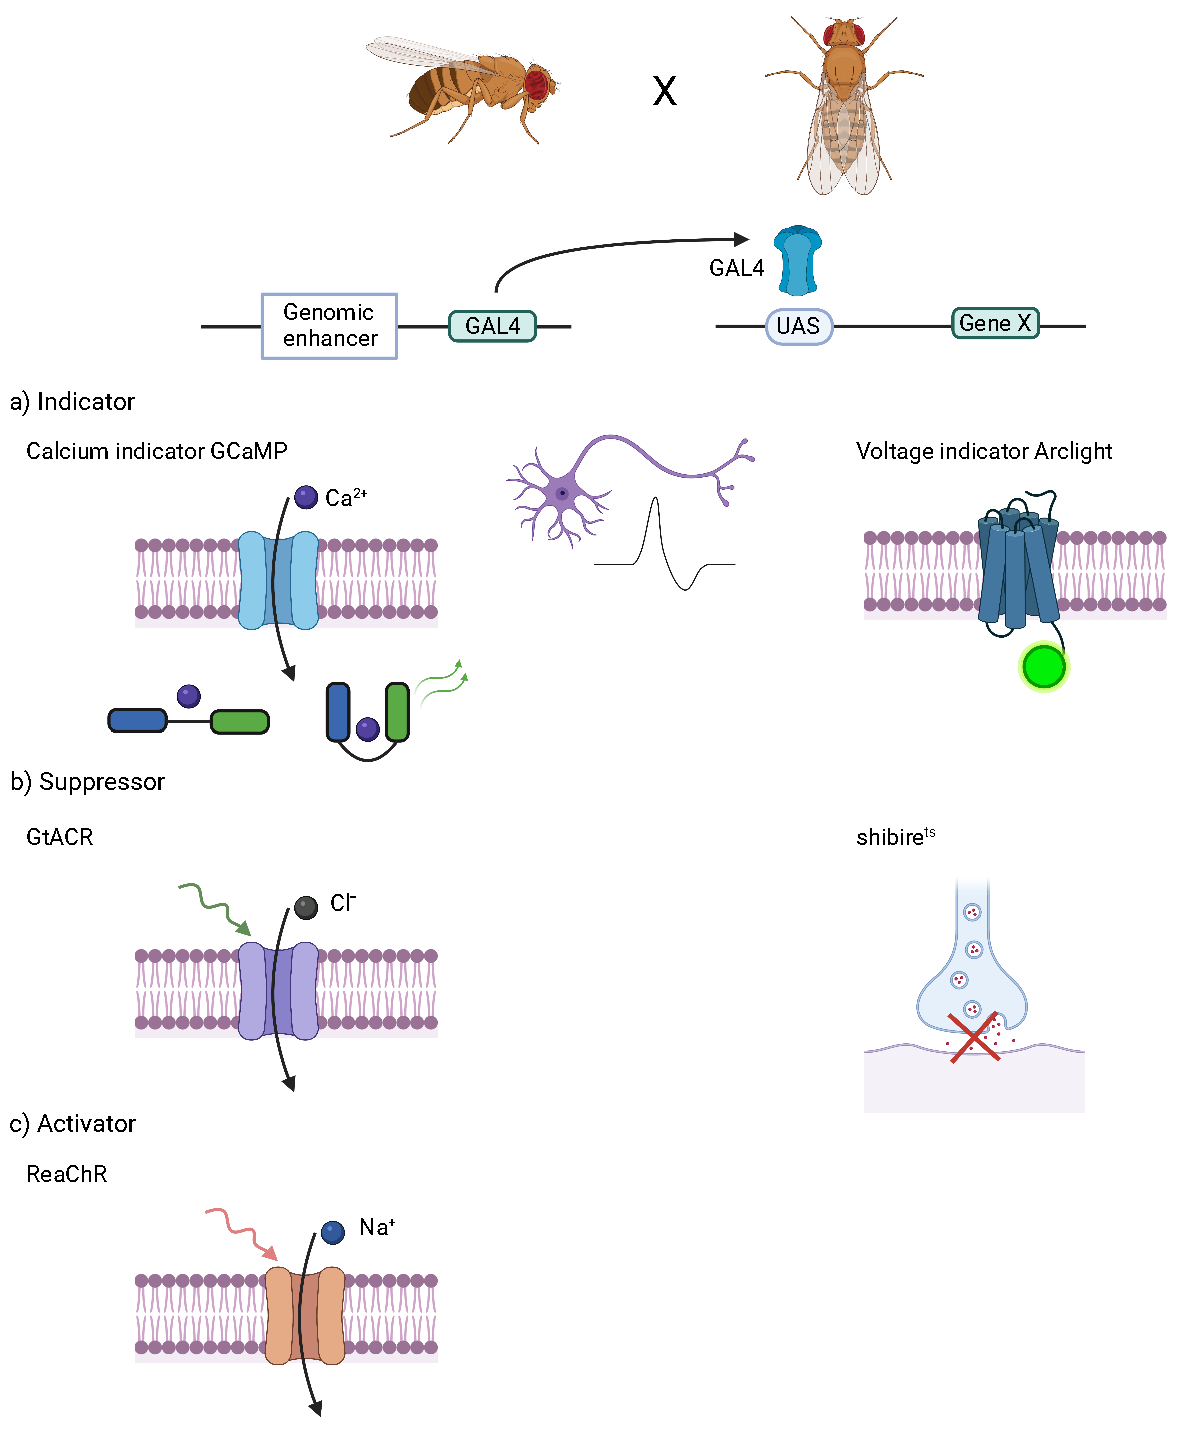
\includegraphics[scale=0.8]{gal4uasfigure}
\caption[Genetic tools for functional manipulations in \textit{Drosophila}] {The Gal4-UAS system is used to express a gene of interest in a specific subset of neurons. (a) Calcium indicator is used to record neural activity using intracellular calcium concentration. Voltage indicator is used to optically record membrane potential changes in the neuron. (b) Neural activity can be suppressed by expressing light sensitive chloride channels or by blocking synaptic transmission via expression of temperature-sensitive $shibire^{ts}$. (c) Neurons can be activated via expression of light-sensitive cation channels. (modified from \cite{Borst2009})}
\label{fig:gal4uas}
\end{figure}
\subsection{Calcium Indicator : GCaMP for recording changes in intracellular calcium}
To record neuronal activity, one can use GAL4-UAS system to express GFP in the required neuron, and then use somatic patch recording to record neural activity from the neuron \parencite{Wilson2004, Joesch2008}. However, neurons in the optic lobe of \textit{Drosophila} are often too small in size for successful electrophysiological recording. To overcome this we can use calcium indicators as proxy for neuronal activity (figure  \ref{fig:gal4uas}a). 

Neural activity causes rapid changes in intracellular free calcium \parencite{Baker1971, Sabatini2002, Egelhaaf1995}. We can thus express genetically encoded calcium indicators (GECIs) which changes its fluorescence according to the change in concentration of intracellular calcium. GECIs typically consist of a calcium-binding domain - calmodulin, calmodulin-binding peptide M13, and a reporter element which is based on either a single fluorescent protein or two fluorescent proteins \parencite{Broussard2014}. In the case of single fluorescent protein for example in GCaMPs, calmodulin (CaM) binds the M13 peptide in the presence of calcium. This coupling results in conformational changes in the fluorescent protein, resulting in change in fluorescence intensity \parencite{Nagai2001}. In the case of two fluorescent proteins, conformational changes lead to Fluorescence Resonance Energy Transfer (FRET) between two fluorescent proteins with overlapping excitation and emission spectra \parencite{Miyawaki1997}. In this thesis, we use GCaMP6f  \parencite{Chen2013} in combination with two-photon microscopy for recording neural activity.

\subsection{Voltage Indicator : Arclight for recording changes in neuronal membrane potential}
In order to measure the membrane potential changes in neurons, electrophysiology has been the most frequently used method. However, due to the small size of neurons in the optic lobe, single-cell electrophysiological recordings of these neurons have been difficult. Genetically encoded voltage indicators (GEVIs) have evolved as powerful tools for recording changes in neuronal membrane potentials. Optical methods of monitoring brain activity are appealing because they allow simultaneous, noninvasive monitoring of activity in many individual neurons and different parts of the brain. 

We use a fluorescence protein (FP) voltage sensor called Arclight \parencite{Jin2012}. Arclight is based on the fusion of voltage sensing domain of \textit{Ciona intestinalis} voltage sensitive phosphatase \parencite{Murata2005} and the fluorescent protein super ecliptic pHluorin with an A227D mutation. Arclight's fluorescence decreases with membrane depolarization and increases with membrane hyperpolarization. We used Arclight in combination with two-photon imaging to record changes in neuronal membrane potential.

\subsection{Suppressor : $shibire^{ts}$, GtACR for silencing neuron}
In order to understand the principles of information processing in a neural circuit, along with recording neural activity we would also like to either suppress or activate neural activity in other neurons in the circuit. Inactivation and activation of genetically defined cell types help establish causal relations in specific group of neurons and neural circuit. There are several tools which allow for inactivation of a neuron. Cell death genes such as \textit{reaper (rpr)} and \textit{head involution defective (hid)} or \textit{grim} induce apoptosis \parencite{Chen1996, Grether1995}.  The tetanus toxin light chain (TeTxLc) cleaves the synaptic vesicle protein synaptobrevin, and inhibits neurotransmitter exocytosis at chemical synapses \parencite{Sweeney1995}. The expression of Kir - an inwardly rectified potassium channel causes neurons to hyperpolarize, resulting in suppressed excitability \parencite{Johns1999}. While using Gal4-UAS system to express these effectors provide effective control over the functionality of the targeted neurons, it also creates some unwanted problems. First, because most enhancers are active at several stages of development, it is difficult to avoid the toxic effects of expressed gene product on development. Second, if particular neurons are eliminated during development, their loss in function may be compensated by some other neuron, hence making interpretation of results difficult. third, it is not possible to observe acute effect elicited by the temporal inactivation of particular neurons. To overcome these limitations, we can use conditional effector proteins like $shibire^{ts}$ \& GtACR (figure  \ref{fig:gal4uas}b), which is activated by higher temperature \& light respectively. 

\textit{Drosophila shibire} encodes the protein dynamin, which is involved in the process of endocytosis and is essential for vesicle recycling. The dominant-negative temperature sensitive allele $shibire^{ts}$ is defective in synaptic vesicle recycling at restrictive temperature ($>29\degree C$) which results in rapid and reversible inhibition of synaptic transmission \parencite{Kitamoto2001}. In \textit{Drosophila}, \cite{Joesch2010} showed that flies expressing $shibire^{ts}$ if exposed to persistent heat-shock for one hour at restrictive temperature $(37\degree C)$, the output of affected cells is suppressed for several hours. This experimental method gives us a longer time duration, which allows us to record neural activity from the fly while the activity from the neuron expressing $shibire^{ts}$ is suppressed. However, we get this extra time duration at the cost of losing reversibility of activity.

The tools we have mentioned above allows for a cell-type-specific neuromodulation. However, in addition to the cell-type-specificity we would also like to have temporally accurate and reversible neuromodulation. \textit{Guillardia theta} Anion Channel Rhodopsins (GtACR1 and GtACR2) can provide us with these additional advantages \parencite{Govorunova2015}. GtACRs impart strong light-gated chloride conductance and is much more light-sensitive than Halorhodopsin class of chloride pumps. In particular with respect to the fly visual visual system, we used GtACR1 since its activation spectrum is shifted towards longer wavelengths with respect to five of the six \textit{Drosophila} rhodopsins (except rhodopsin 6) \parencite{Mauss2017, Mohammad2017}. Thus, we can use Gal4-UAS system to express GtACR in neurons we want to hyperpolarize \& silence the neural activity. Simultaneously, we can express GCaMP in downstream neurons using LexA-lexAop system \& record their neural activity, while silencing the neurons expressing GtACR. 

 
\subsection{Activator : ReaChr for activating neuron}
Along with using GCaMP for imaging, $shibire^{ts}$ or GtACR for suppressing neural activity, we would also like to have a tool for activating neuron. Ideal method for activation requires excellent temporal control. Light-gated cation channels - Channelrhodopsins(ChRs) can be used for this purpose (figure  \ref{fig:gal4uas}c). ChRs are light-gated, non-specific cation channels that allow selective depolarization of genetically targeted cells. Here we have used red-activatable ChR (ReaChr), a variant of ChR \parencite{Lin2013, Busch2018}. 

Therefore by combining the use of GCaMP for calcium imaging and GtACR for suppression or ReaChR for activation, we can better understand the functions of neurons present in a given neural circuit.

\section{Neural communication}
Camillo Golgi's silver-stain method made it possible to visualize the nervous system in tissue samples under the light microscope around 1873. Santiago Ramón y Cajal in 1888 described the nervous system as a network of individual cells. About a decade later, in 1897, the term 'synapse', derived from the Greek word 'synapsis' (meaning 'conjunction'), was used to describe the connections between two neurons. Neurons form networks where they communicate via synapses. Two types of synapses exist: 1) Electrical synapses 2) Chemical synapses

\subsection{Electrical synapses}
In electrical synapses, two cells are directly connected by cluster of intercellular channels called gap junctions \parencite{Bennett2004}. The gap junctions provide a conductive pathway for electrical current to spread between cells that are interconnected. Consequently, electrical currents underlying action potentials or graded potentials directly propagate to postsynaptic neurons, with a similar time course to presynaptic signals. Additionally, since electrical signals propagate bidirectionally, signalling events generated in the postsynaptic cells also spread to the presynaptic cells. In \textit{Drosophila}, electrical synapses are widely distributed throughout the nervous system and are essential to neuronal function \parencite{Ammer2022}.

%In order to guide animal behavior, neurons perform a wide range of computations. Neurons encode information via graded changes in membrane potential or action potential frequency.


\subsection{Chemical synapses}
Neurons communicate mostly via chemical synapses (figure  \ref{fig:chemicalsynapse}) which requires the release of neurotransmitters. When the presynaptic membrane is sufficiently depolarized, voltage-gated calcium channels open and allow $Ca^{2+}$ to enter the cell \parencite{Luo2020}. Calcium entry leads to the fusion of synaptic vesicles with the membrane and release of neurotransmitter molecules into the synaptic cleft \parencite{Chapman2002}.  As neurotransmitters diffuse across the synaptic cleft, they bind to receptors in the postsynaptic membrane, causing postsynaptic neuron to depolarize or hyperpolarize, passing the information from pre to postsynaptic neurons \parencite{Maio2008}. Voltage to calcium transformation in neurons is therefore a crucial step in neural information processing and neural computation. 

\begin{figure}
\centering
\hspace*{-1cm} 
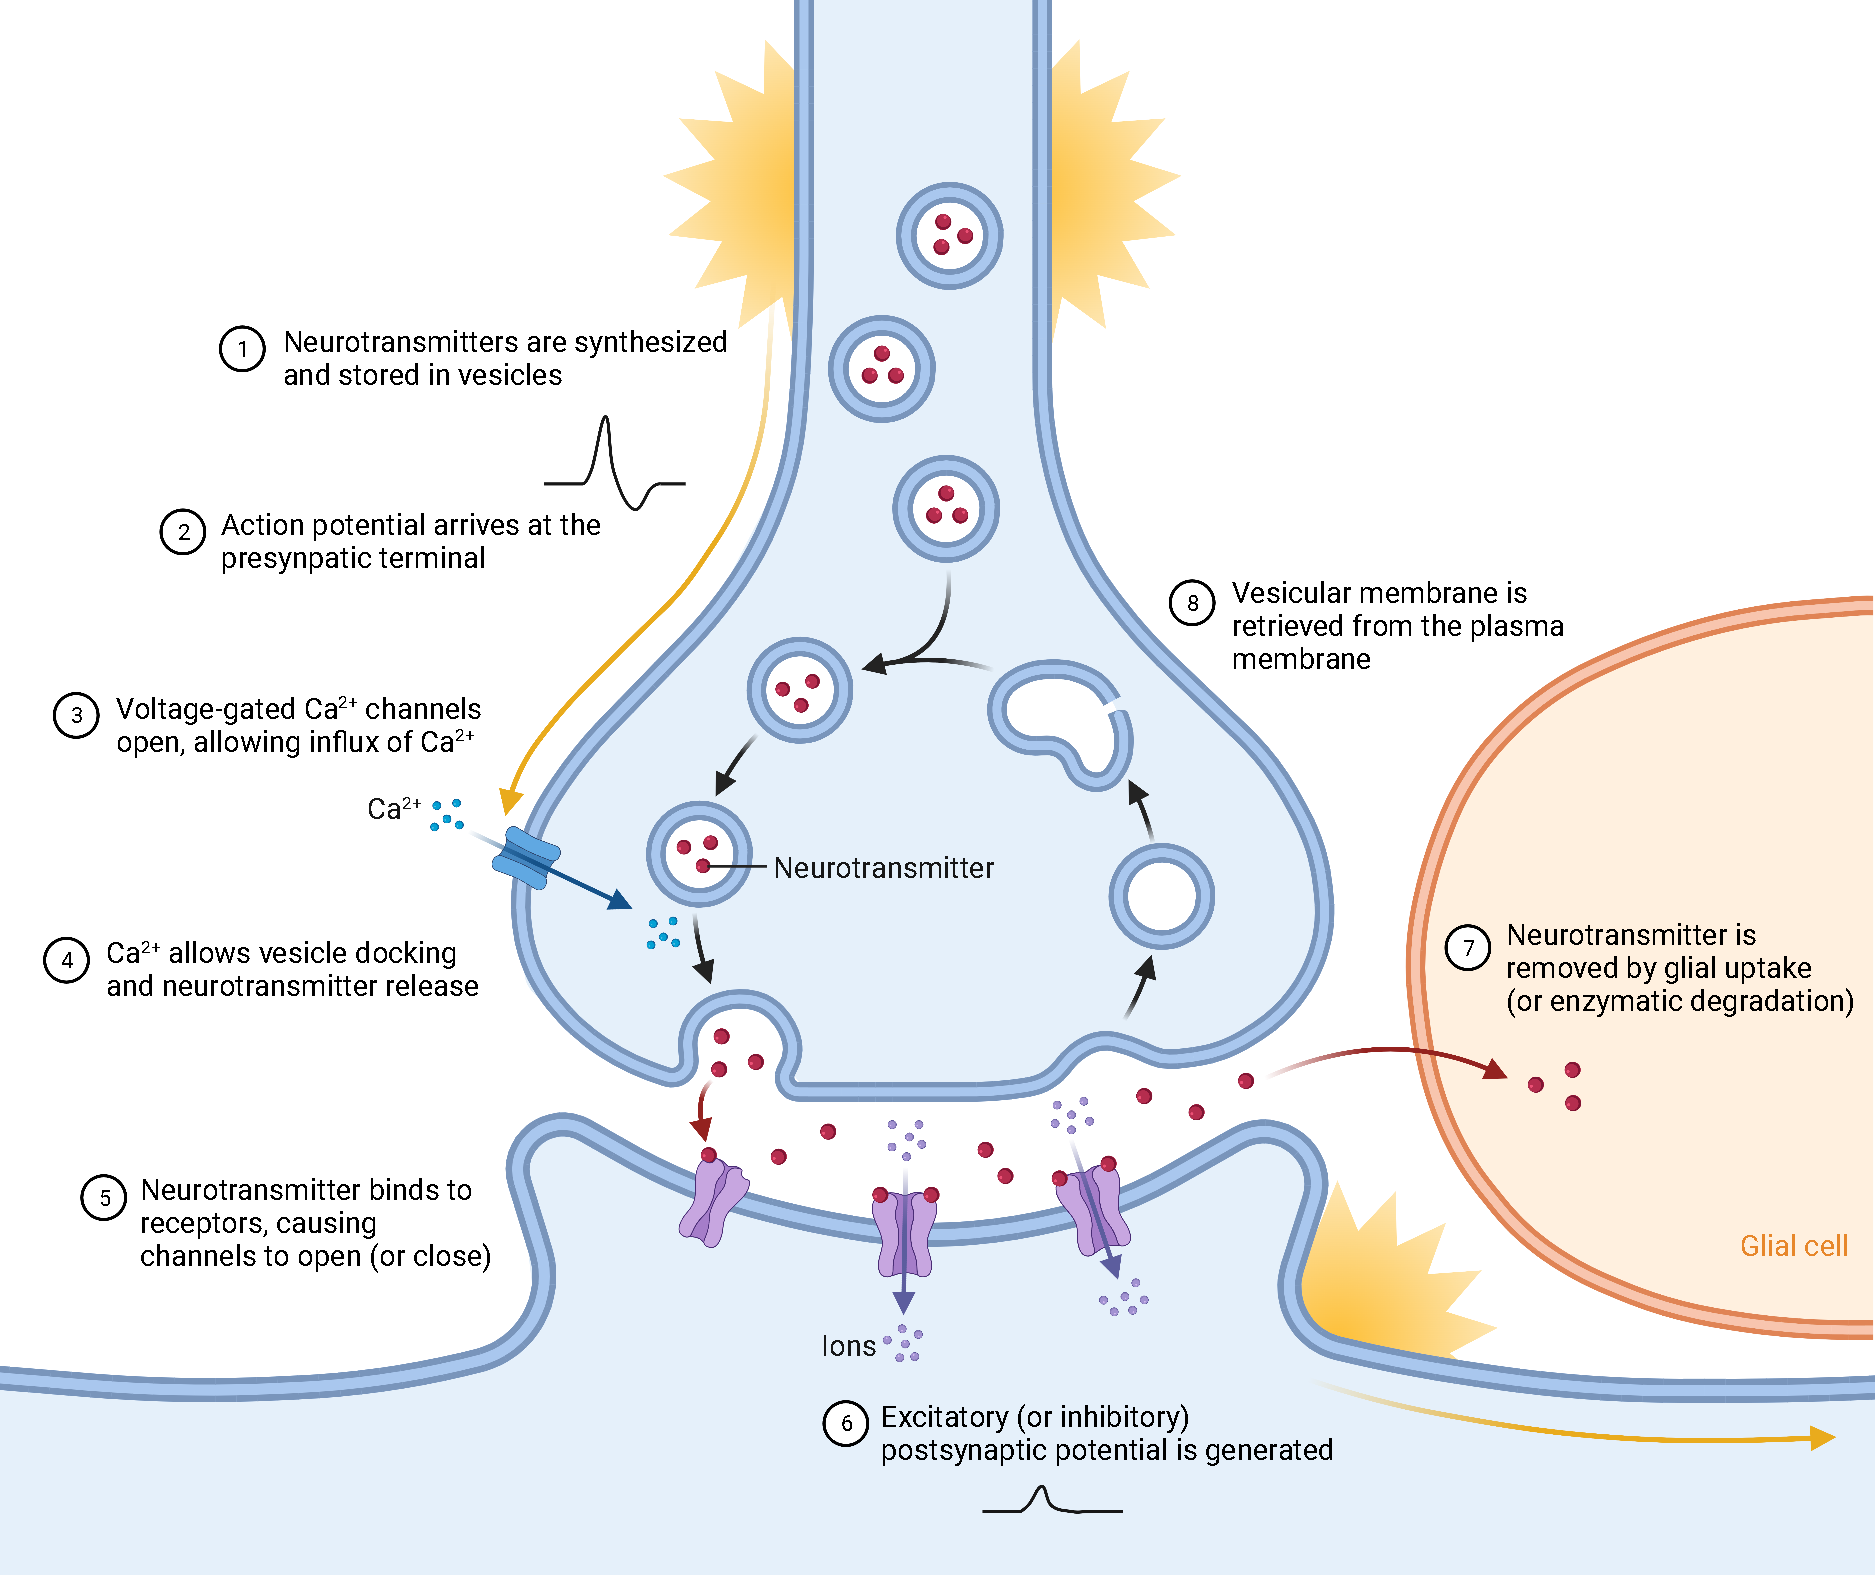
\includegraphics[scale=0.5]{Chemical_Synapse}
\caption[Chemical synapse: steps of synaptic transmission] {Chemical synapse: steps of synaptic transmission. (1) Synthesis and storage of neurotransmitter in the vesicles. (2) Depolarization in the presynaptic terminal causes (3) voltage-gated calcium channels to open and allow influx of calcium ions. (4) High concentration of calcium ions trigger the fusion of neurotransmitter filled vesicles with the presynaptic membrane and release of neurotransmitters into the synaptic cleft. (5) Neurotransmitters released in the synaptic cleft bind to receptors in the postsynaptic membrane leading to (6) excitatory or inhibitory postsynaptic potential. (figure created with \href{https://app.biorender.com/biorender-templates}{Biorender.com})}
\label{fig:chemicalsynapse}
\end{figure}

\subsection{Voltage-gated ion channels}
Voltage-gated ion channels are transmembrane proteins that allow certain inorganic ions to cross cell membranes (figure  \ref{fig:vgatedionc}). Generally, these channels consist of two distinct but functionally coupled transmembrane domains: the voltage sensing domain and the pore domain. The voltage sensing domain changes the confirmation of the pore domain in response to changes in transmembrane potential, allowing selected ions to flow down their electrochemical gradient. 

\paragraph{Voltage-gated calcium channels}
Voltage-gated calcium channels mediate depolarization-induced calcium influx that drives release of neurotransmitter. The $\alpha1$-subunit of the voltage-gated calcium channels forms the ion-conducting pore, which makes it distinct from other calcium channels. Three families of genes encode $\alpha1$ subunits. \textit{Drosophila} genome has one $\alpha1$ subunit gene in each family: $\alpha1D$ ($Ca_{v}1$), cac ($Ca_{v}2$), and $\alpha1T$ ($Ca_{v}3$) \parencite{Littleton2000, King2007}. In \textit{Drosophila} antennal lobe projection neurons, cac ($Ca_{v}2$) type and $\alpha1T$ ($Ca_{v}3$) type voltage-gated calcium channels are involved in sustained and transient calcium currents, respectively \parencite{Gu2009, Iniguez2013}.

\paragraph{Voltage-gated sodium channels}
In neurons, voltage-gated sodium channels play a crucial role in the initiation and propagation of action potentials \parencite{Hodgkin1952}. Sodium channels are activated and deactivated within milliseconds when the membrane is depolarized by a few millivolts. There are at least ten genes in mammals that encode these large membrane proteins. In contrast, \textit{paralytic (para)} is the only voltage-gated sodium channel gene described in Drosophila. Loss of \textit{paralytic (para)} reduces neuroblast progeny cell number in \textit{Drosophila} \parencite{Piggott2019}.

\paragraph{Voltage-gated potassium channels}
Voltage-gated potassium channels are transmembrane channels specific for potassium ions. They play a crucial role in returning the depolarized cell to its resting membrane potential, after each action potential. Voltage-gated potassium channels are the most diverse family of voltage-gated ion channels in the human genome, with 40 members for $\alpha$ subunit grouped into 12 families \parencite{Gutman2005}. The first voltage-gated potassium channel discovered in the \textit{Drosophila} was \textit{Shaker} \parencite{Papazian1987}. Afterwards, three additional \textit{Shaker} like voltage-gated potassium genes were identified in \textit{Drosophila}: \textit{Shab}, \textit{Shaw} and \textit{Shal} \parencite{Covarrubias1991}. 

\begin{figure}
\centering
\hspace*{-1cm} 
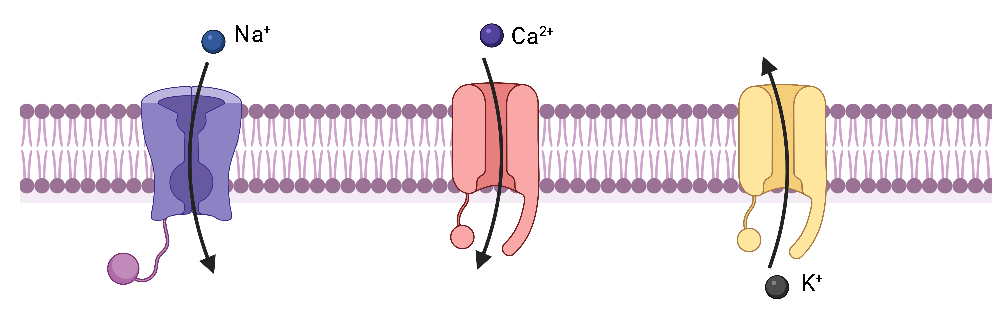
\includegraphics[scale=0.85]{voltagegatedionchannels}
\caption[Voltage-gated ion channels] {Voltage-gated ion channels: The sodium channels allow $Na^{+}$ ions to enter into the cell. The calcium channels allow $Ca^{2+}$ ions to enter into the cell. The potassium channels allow efflux of the $K^{+}$ ions.}
\label{fig:vgatedionc}
\end{figure}


\section{Fly motion vision system}
\textit{Drosophila} visual processing pathway is comprised of retina, lamina, medulla, lobula and lobula plate, each arranged in columnar, retinotopic fashion (figure \ref{fig:opticlobe}a) \parencite{Fischbach1989}. If one were to record from a single photoreceptor in the retina, it would show similar response to a patch of moving image irrespective of the direction of motion: meaning it is not direction-selective. However, if one records around 4 synapses downstream, Lobula Plate Tangential Cells (LPTCs) depolarise in response to a patch of image moving in its preferred direction and hyperpolarize if the image moves in opposite direction or the null direction (figure \ref{fig:opticlobe}b). HS (Horizontal System) cells for example are responsive to horizontal motion \parencite{Schnell2010}, while VS (Vertical System) cells are responsive to vertical motion \parencite{Joesch2008}. LPTCs, however integrate over large parts of visual fields, i.e. they are not local motion detectors. Hence, the natural question arises: which cells are the local motion detectors? 

\begin{figure}
\centering
\hspace*{-1cm} 
\includegraphics[scale=0.85]{fly_optic_lobe}
\caption[Fly optic lobe] {Fly optic lobe}
\label{fig:opticlobe}
\end{figure}

The answer to the above question is: T4 and T5 are first local motion detectors found in the \textit{Drosophila} ON and OFF motion vision pathway respectively. Four sub-population of T4a-d and T5a-d cells tuned to the four cardinal directions and projecting to the four layers in the lobula plate can be found within each column \parencite{Maisak2013}. This leads to next question: what makes T4 and T5 direction selective? To answer this question, we need to investigate the cells which are present in between the non-direction-selective photoreceptors in the retina and direction-selective T4, T5 cells in Medulla and Lobula respectively (figure \ref{fig:opticlobe}c, d). The columnar cell types of the lamina, medulla, lobula and lobula plate have all been identified and described \parencite{Fischbach1989, RamonyCajal1915}.  

\paragraph{Lamina}
Lamina is organized in an array of $\sim 750$ retinotopic columns (also called 'cartridges'). Each column corresponds to $\sim 5\degree$ discrete sample of the visual world. Light sensitive photoreceptors, R1-6 project their axons into each lamina column. Two other photoreceptors, R7 \& R8 pass thorugh lamina and synapse in specific layers of medulla. Along with photoreceptor axons, lamina includes 5 lamina output neurons (L1-L5), six putative feedback neurons (T1, Lat, Law1, Law2, C2, C3) and one lamina intrinsic neuron (Lai). Lamina columnar monopolar neurons, L1-L5 send their axonal projections into specific layers of the medulla. \parencite{Fischbach1989, Tuthill2013}. 

\paragraph{Medulla}
Medulla consists of more than 60 different cell types in a single column. They can be clustered into different groups based on their anatomy. Medulla intrinsic ('Mi') neurons connect different layers of the medulla to each other. Trans-medulla ('Tm') neurons connects specific layers of medulla to various layers in the lobula. Trans-medulla Y ('TmY') neurons connect specific layers of the medulla to various layers in the lobula and lobula plate. The medulla consists of 10 layers, M1 to M10. Directions-selective cell T4 connects medulla layer 10 to the four layers of lobula plate.

While the circuit was known, the small size of these neurons made electrophysiological recordings difficult. Only after the advent of modern 2-photon imaging in combination with using Gal4-UAS system to express GCaMP in these cells, it became possible to record neuronal activity from these cells. Experiments over the years using these techniques revealed following interesting results : (a) Visual processing in \textit{Drosophila} occur in two parallel processing pathways for brightness increment (ON) and brightness decrement (OFF) \parencite{Joesch2010, Joesch2013, Strother2014, Eichner2011, Behnia2014} (b) T4 and T5 are first local motion detectors found in the \textit{Drosophila} ON \& OFF motion vision pathway respectively. Four sub-population of T4a-d and T5a-d cells tuned to the four cardinal directions and projecting to the four layers in the lobula plate can be found within each column \parencite{Maisak2013}. 


\subsection{Parallel ON and OFF processing pathways}
In striking similarity to mammalian retina \parencite{Masland2012}, visual processing in \textit{Drosophila} occurs in two parallel ON and OFF processing pathways \parencite{Borst2015}. The ON pathway transmits information about brightness increments, while the OFF pathway transmits information about brightness decrements. In order to understand split of photoreceptor (R1-R6) signals into ON and OFF pathway, studies have been done blocking Laminar monopolar cells, while simultaneously recording from downstream LPTCs neuron. While blocking L1 neurons resulted in specific reduction of LPTC's response to ON stimulus (brightness increment), blocking L2 neurons resulted in specific reduction of LPTC's response to OFF stimulus (birghtness decrement) \parencite{Joesch2010}. In behavioral experiments, walking flies were unable to follow either ON or OFF motion when either L1 or L2 was blocked respectively \parencite{Clark2011, Maisak2013}. The flies become completely motion-blind if both L1 and L2 are permanently hyperpolarized (via Kir2.1) \parencite{Tuthill2013, Bahl2013}. These experiments together suggests that L1 pathway specifically transmits information about brightness increments to downstream ON motion detector, and L2 pathway specifically transmits information about brightness decrements to downstream OFF motion detector. 

\subsection{T4 and T5 cells}
Based on previous studies from \parencite{Fischbach1989, Buchner1984}, T4 and T5 were long thought to be the prime candidates for local motion detectors in the ON and OFF pathway respectively. However, due to its small size it was difficult to do electrophysiological recordings from T4 and T5 cells. This problem was solved using combination of 2-photon imaging and Gal4-UAS system to express GCaMP in T4, T5 cells to record its neural activity in response to the ON and OFF stimuli. Stimulating the flies in four cardinal directions (front-back, back-front, upwards and downwards), \cite{Maisak2013} recorded direction selective activity from T4/T5 cells. Four sub-population of T4a-d and T5a-d cells tuned to the four cardinal directions and projecting to the four layers in the lobula plate were found within each column. Further, T4 were found to respond specifically to ON stimulus and T5 were found to respond specificaly to OFF stimulus. Blocking T4 and T5 cells led to a complete loss of motion response in lobula plate tangential cells \parencite{Schnell2012}, of the optomotor response of tethered walking flies \parencite{Bahl2013}. Specific blocking of T4 cells led to reduction in LPTC and optomotor responses to ON stimulus selectively. While specific blocking of T5 cells led to reduction in LPTC and optomotor responses to OFF stimulus selectively. These results together suggest T4 and T5 to be the elementary motion detector for ON and OFF pathway respectively \parencite{Maisak2013}.      

\section{Neural circuit underlying direction selectivity}
Having identified T4 and T5 as the elementary local motion detectors, the next question which arises is which cells provide synaptic inputs to T4 and T5 cells. Electron Microscopy (EM) studies \parencite{Shinomiya2019, Takemura2017} provided answer to this question. \cite{Shinomiya2019} used FIB-SEM (Focused Ion Beam Serial Electron Microscope) to record a volume of the optic lobe comprising of seven columns of the medulla, lobula and lobula plate. They identified all the different neuron types providing inputs to the T4 and T5 cells. T4 cells receive input from Mi1, Tm3, Mi4, Mi9, C3, CT1 and TmY15. T5 cells receive input from Tm1, Tm2, Tm4, Tm9, CT1, TmY15, LT33 and Tm23. T4 and T5 cells' dendrites span over several columns along the preferred direction of the motion. The authors could also locate where the different cell type synapse onto the dendrites of T4 and T5. For example for T4c with preferred direction of motion as upwards receives input from Mi1, Tm3 and TmY15 in the central part of its dendrite, from Mi9 and T4c on the ventral part and from Mi4, C3 and CT1 on the dorsal part of its dendrite [figure \ref{fig:t4t5inputsynapses} top]. For T4d with preferred direction as downwards, it receives input from Mi1, Tm3 and TmY15 in the central part, from Mi9 and T4d on the dorsal part and from Mi4, C3, CT1 on the ventral part of its dendrite. In summary, all T4 subtypes receive inputs from Mi1, Tm3 and TmY15 in the central part, from Mi9 on the preferred side (i.e. the side from which a preferred direction stimulus approaches) and from Mi4, C3 and CT1 on the null side (i.e. the side from which a null direction stimulus approaches) of their dendrite. Similarly, all T5 subtypes receive inputs from Tm1, Tm2 and Tm4 on the central part, Tm9 on the preferred side and CT1 on the null side of their dendrite [figure \ref{fig:t4t5inputsynapses}]. %a figure showing summary of different inputs.    

\begin{figure}[h]
\centering
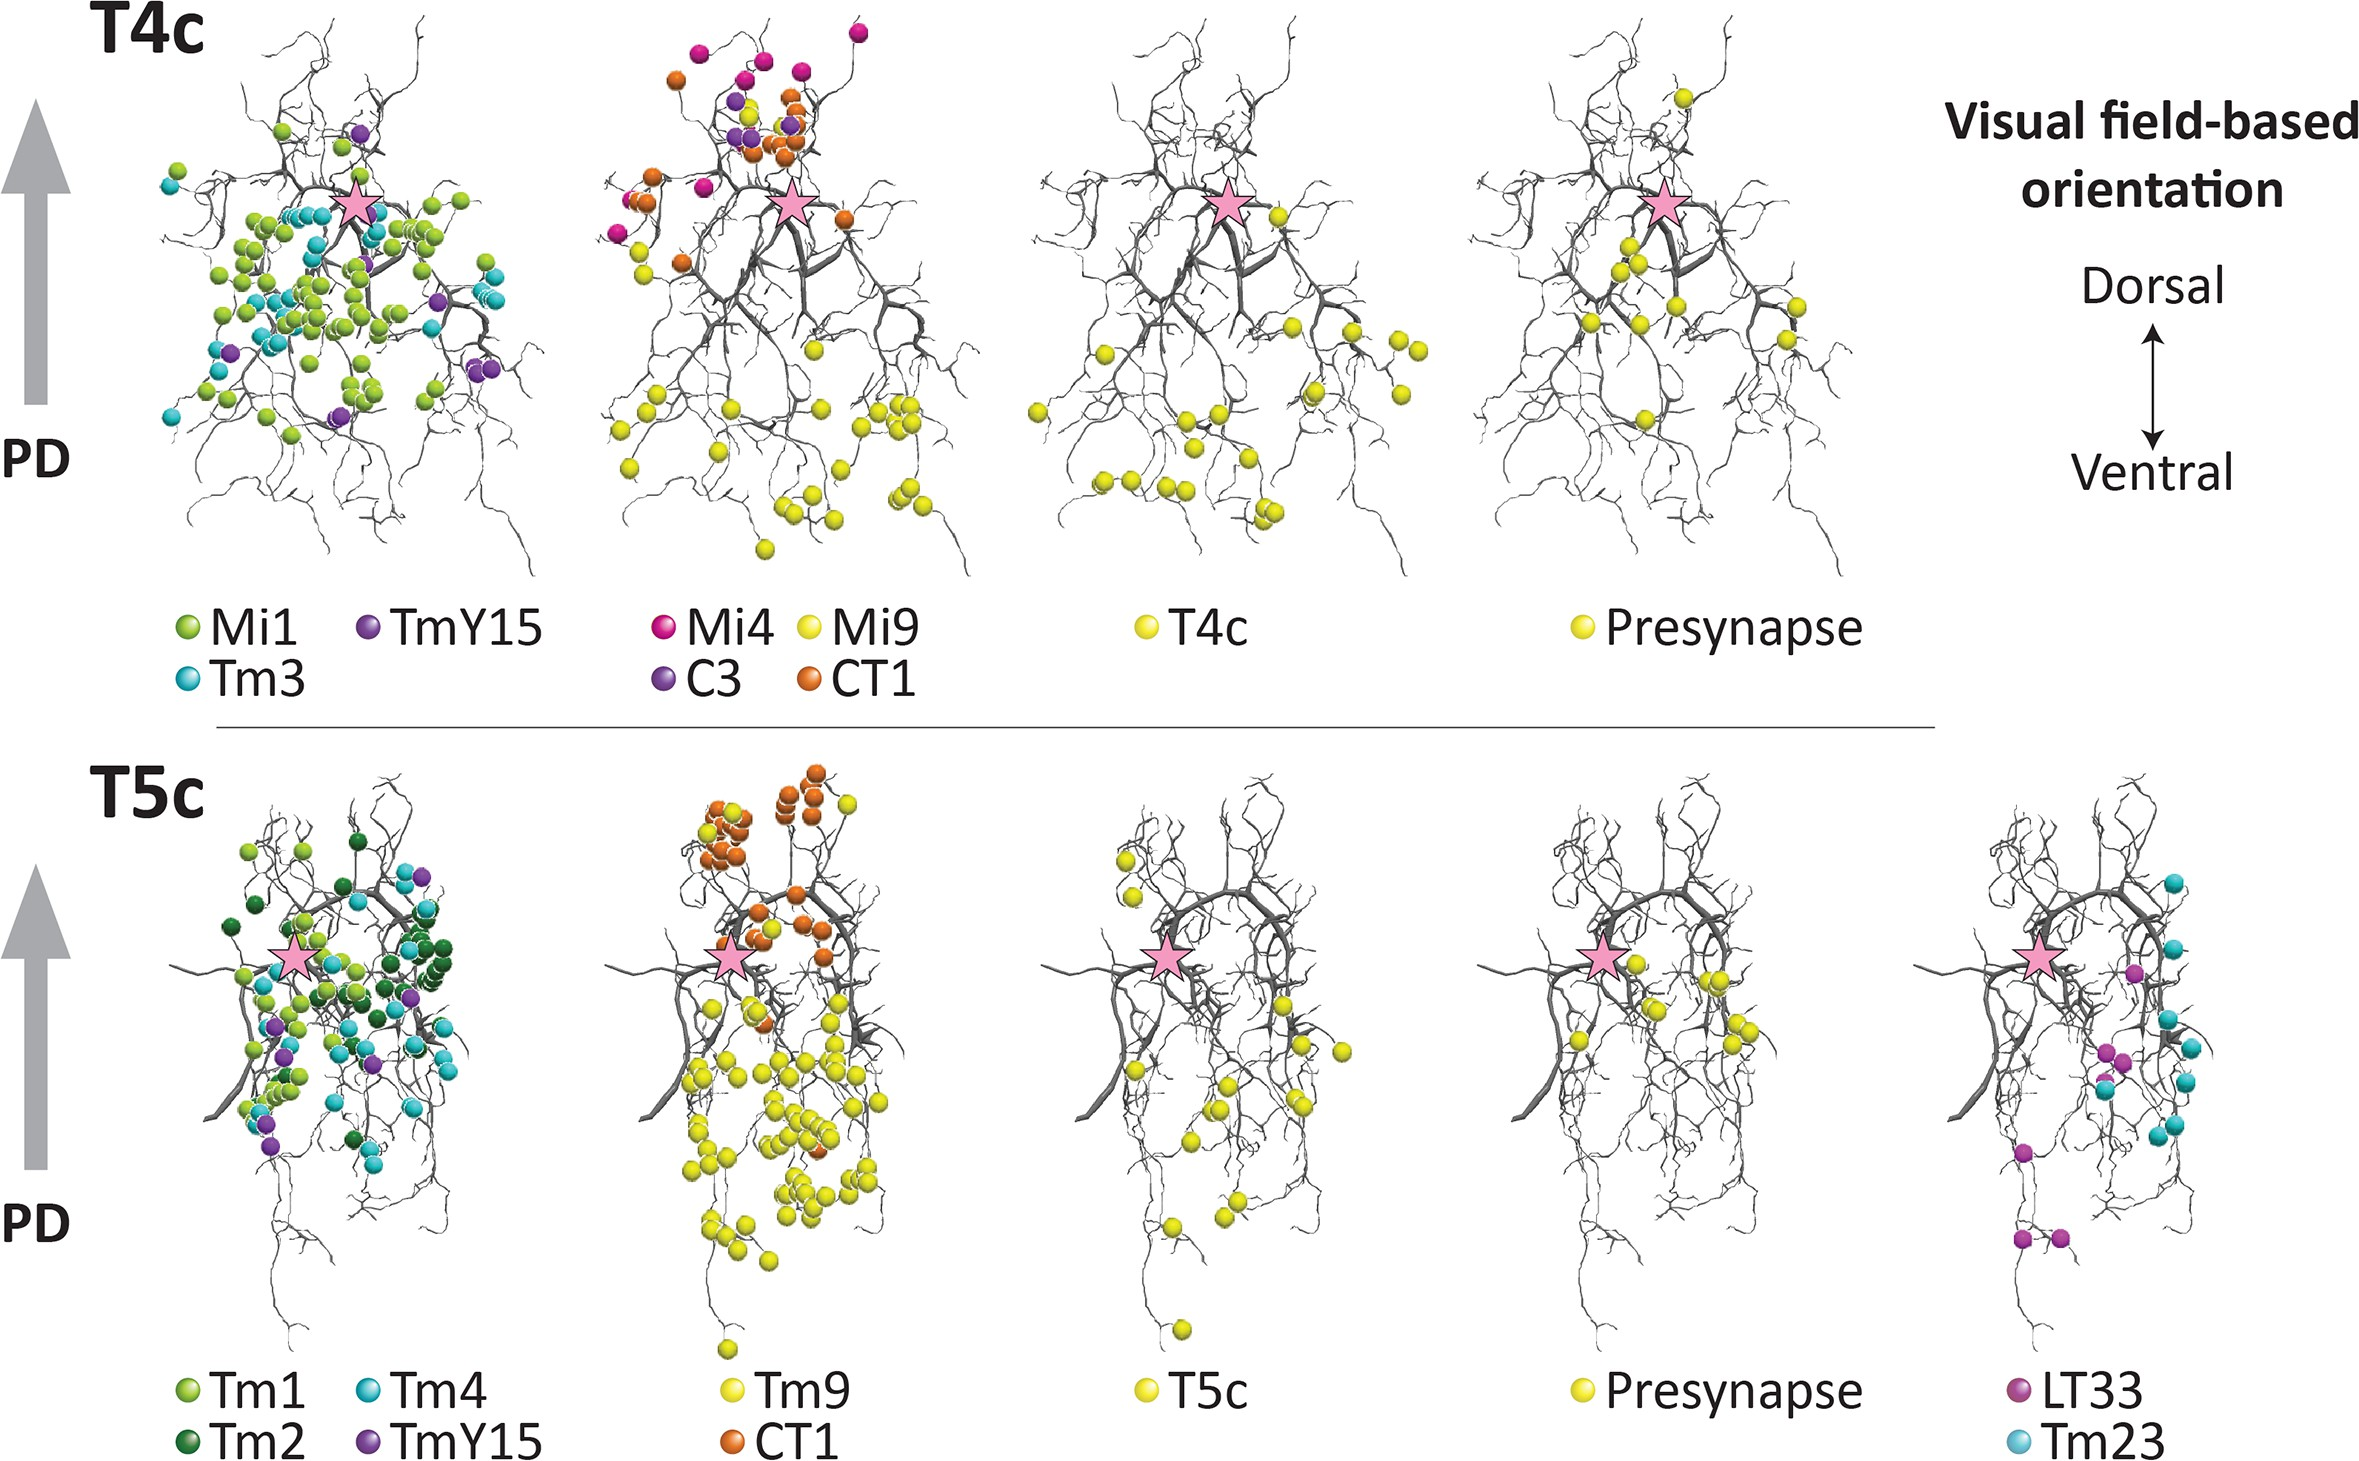
\includegraphics[scale=0.2]{t4t5inputsynapses}
\caption{t4t5inputsynapses}
\label{fig:t4t5inputsynapses}
\end{figure}

Most of these input elements have been characterised physiologically \parencite{Arenz2017, Serbe2016, Strother2017, Meier2019, Borst2020}. None of these cells were found to be direction-selective. Hence, we can conclude that T4 and T5 are the first elementary motion detector found in the ON and OFF pathway respectively, and thus represents an important processing stage where direction is computed.    

\section{Neural algorithm underlying direction selectivity}
The underlying mechanisms generating direction selectivity and the neural correlates implementing these mechanisms have not been yet fully understood. Classically two opposing models have been proposed for implementation of direction selectivity. Both these model use two input lines, where one of the input line has been asymmetrically delayed compared to the the other, which is then followed by a non-linear interaction. The Hassenstein-Reichardt (HR) model proposes a Preferred Direction (PD) enhancement : the signal on the preferred side is delayed and is subsequently amplified using multiplication of the signal from the other input line [\textbf{Figure}]\parencite{Hassenstein1956}. The Barlow-Levick (BL) detector however, proposes a Null Direction (ND) suppression : the signal on the null side is delayed and divides the signal from the other input resulting in suppression \parencite{Barlow1965} . \cite{Haag2016a} used apparent motion stimuli to show that both the mechanisms i.e. PD enhancement and ND suppression is used by T4 and T5 cell to produce a direction selective response. In our \textbf{manuscript1} - \parencite{Haag2017}, we showed that all four subtypes of T4 and T5 indeed uses both PD enhancement and ND suppression to produce direction selective responses. Therefore, a new model combining both PD enhancement on the preferred side and ND suppression on the null side was proposed. The next important task now is to identify neural correlates implementing these mechanisms. 

The model requires a fast input at the center, slow input providing excitation on the preferred side and slow input providing suppression on the null side. Interestingly, from the anatomical and functional characterization of input data we have discussed earlier, we could predict the input neurons for T4 providing these three kind of inputs. Mi1 is a fast neuron providing input at the central part of dendrite, thus a candidate for central fast input. Mi9 is a slow neuron providing input on the preferred side of the dendrite, hence a candidate for slow excitatory input. Mi4, C3 and CT1 are slow neurons providing input on the null side of the dendrite. In \textbf{manuscript2} we have expressed GtACR or ReaChr to silence or activate input neurons respectively. Simultaneously, we express GCaMP in the downstream T4c/T5c neurons. These experiments together help us understand the functional contribution of each of these input neurons to direction selective signals in T4.




